\section{Dettagli Implementativi}

% Just report interesting / non-trivial / non-obvious implementation details.

% This section is expected to be short in case some documentation (e.g. Javadoc or Swagger Spec) has been produced for the software artefacts.
% %
% This this case, the produced documentation should be referenced here.

Il progetto \'e stato documentato (TODO) tramite Javadoc all'interno del codice. \'E per\'o importante evidenziare come la documentazione sia relativa alle sole componenti pubbliche delle classi. Questa scelta deriva dalla convinzione, adottata da molti sviluppatori, secondo la quale un buon codice debba essere `parlante' e non necessiti quidi descrizioni se non relativamente alle funzionalit\'a che possano essere chiamate esternamente.

\subsection{Traduzione dei messaggi}
Una funzionalit\'a che si intende descrivere \'e relativa al marshalling ed un-marshalling dei messaggi dal client JADE agli agenti Jason.\\
Come gi\'a descritto, \'e stata definita una ontologia del sistema per la corretta descrizione delle operazioni e dei loro `target'. La `traduzione' dei messaggi non \'e per\'o logicamente parte dell'ontologia. Allo scopo di creare una struttura pi\'u logicamente corretta si \'e quindi crata una classe di utilities utili alla trasformazione dei messaggi dal formato utilizzato all'interno del client (basato su classi/oggetti) a quello utilizzato dagli agenti Jason (basato invece su Terms, Literals, etc.). Queste utilities sono quindi richiamate ogni qualvolta sia necessario inviare un messaggio dal client ad un agente del magazzino o, viceversa, quando una risposta venga ricevuta. Uno schema della logica appena descritta \'e visibile in Figura \ref{fig:message-translation}.
\begin{figure}[!ht]\centering
    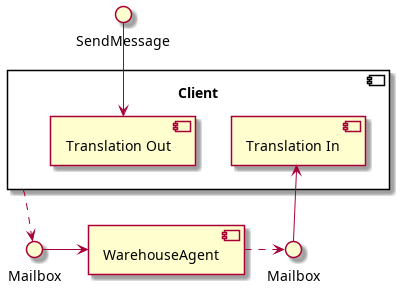
\includegraphics[width=.7\textwidth]{section/implementation/figure/message-translation.png}
    \caption{Rappresentazione schematica del processo di traduzione dei messaggi in ingresso ed in uscita. Quando un messaggio deve essere inviato dall'agente lato client, questo viene innanzitutto tradotto/marshallato dal sistema per poi essere inviato. Viceversa, alla ricezione di un messaggio, questo viene tradotto dal formato utilizzato nel magazzino a quello utilizzato dal client, per poi essere infine utilizzato dal sistema.}
    \label{fig:message-translation}
\end{figure}

\subsection{Reinvio dei messaggi}
Come gi\'a detto, il sistema permette un reinvio dei messaggi in caso di un possibile errore di rete. Allo scopo di ottenere questa caratteristica \'e stato creato un behaviour (all'interno dell'agente di utility Communicator) che periodicamente si occupa di reinviare i messaggi per cui non si sia ricevuta risposta. Questa funzionalit\'a richiede quindi di salvare i messaggi di cui si sia tentato l'invio, insieme al loro timestamp, per permetterne un reinvio in caso una risposta non giunga entro il tempo limite. Il sistema si occupa dunque di considerare il parametro `in-reply-to' per validare la ricezione della risposta ad un messaggio.
